\chapter{Karten-Update Strategien}
\label{chapter:map_update}

Dieses Kapitel basiert auf den Ausführungen in Kapitel \ref{chapter:association}. Dabei wurde herausgestellt, dass ein Update der Karte ohne eine zusätzliche Datenbasis in der Nachbehandlung aufgrund einer Vielzahl an Problemen nicht möglich ist. Im Folgenden wird das Problem auf der um die Menge an Punktwolken $\mathbb{C}$ erweiterten Datenbasis neu betrachtet. Dabei wird das Problem selbst neu aufgerollt. Anstelle in einem fertigen Pose-Graphen wie in Kapitel \ref{chapter:loop_closure} beschrieben nach Schleifenschlüssen zu suchen, den Graphen auf Basis der identifizierten Schleifenschlüsse zu optimieren und darauf beruhend ein Update auf einer bereits fertigen Karte durchzuführend wird nun ein inkrementelles Vorgehen angestrebt. Ziel ist die Möglichkeit zu bieten, den Ansatz in einen existierenden, auf einer TSDF-Karte beruhenden, SLAM-Algorithmus zu integrieren. In einer Nachbearbeitung ist es nicht zwingend notwendig die Karte nach jedem identifizierten Schleifenschluss und der darauf beruhenden Graph-Optimierung ein Update der Karte durchzuführend, da die TSDF-Karte selbst für den vorgestellten Optimierungsprozess, der auf den Punktwolken $\mathbb{C}$ beruht, nicht benötigt wird. Innerhalb eines auf der TSDF-Karte operierenden SLAM-Ansatzes wie \cite{HATSDF} ist es allerdings unerlässlich, dass die Karte in jedem Inkrement auf dem neusten Stand ist um eine konsistente Registrierung neuer Daten an die Karte gewährleisten zu können.

Um dieses Ziel zu erreichen, muss nach jedem Inkrement, in dem eine Graph-Optimierung vorgenommen wurde ein Update der bisher erstellten Karte durchgeführt werden. Da eine sichere und lückenlose Ermittlung von Datenassoziationen basierend auf den Posen $\mathbb{P}$ und der TSDF-Karte nicht ohne weiteres möglich ist, ist an dieser Stelle eine andere Herangehensweise an das Problem des Updates gefragt. In einem ersten Schritt wird hier ein \textbf{Greedy (gierig)}-Ansatz gewählt. Ziel eines solchen Ansatzes ist ein Problem auf eine möglichst einfache Weise zu lösen und dabei längere Laufzeiten der gefundenen Lösung in Kauf zu nehmen. Eine möglichst einfache Lösung beim Update der Karte besteht darin zunächst vollständig auf lokale Updates zu verzichten und stattdessen die gesamte Karte zu löschen und neu zu generieren. Dies ist bezogen auf die Laufzeit besonders bei großen Datensätzen keine gute Idee, da auch Teile der Karte vollständig gelöscht und neu generiert werden, die keines Updates bedürfen. Aus diesem Grund wird im weiteren Verlauf dieses Kapitel zusätzlich auf ein partielles, lokales Update der Karte eingegangen und die benötigten Voraussetzungen und Fallstricke beschrieben. Ziel ist hier eine erhebliche Reduktion der Laufzeit. Zunächst wird im folgenden Abschnitt auf das beschriebene globale Update eingegangen.

\section{Globales Update der Karte}
\label{section:global_update}

Dieser Abschnitt befasst sich mit dem beschriebenen Greedy-Ansatz zur Lösung des Kartenupdates. Ziel ist das Löschen der gesamten TSDF-Karte und die nachfolgende Regeneration der Karte basierend auf der erweiterten Datenbasis. Im ersten Schritt wird betrachtet, wie die Karte am effizientesten gelöscht werden kann. Hier lohnt sich eine Betrachtung des Datenflusses zwischen der lokalen und globalen Karte. Dieser wurde in Kapitel \ref{chapter:grundlagen} bereits kurz angeschnitten. Die globale Karte kapselt die Funktionalität zur Serialisierung und Deserialisierung von Daten basierend auf der HDF5-Datei als Speichermedium. Die globale Karte tauscht die benötigten Daten Chunk weise mit der HDF5 aus. Jeder Chunk beinhaltet eine fest definierte Anzahl an TSDF-Gewichten und zugehörigen Werten und deckt einen vorgegebenen Bereich der globalen Karte ab, der über den Index des Chunks definiert ist. Die lokale Karte ist ein 3D Fenster mit vorgegebenen Seitenlängen, welches den aktuell betrachteten Teil der globalen Karte enthält und über die globale Karte wandern kann. Die lokale Karte liefert dabei eine Abstraktion zur globalen Karte. Grundsätzlich werden neue Daten nur über die lokale Karte geschrieben und schlussendlich an die globale Karte zurückgeliefert, die diese gegebenenfalls serialisiert. Dieses Konstrukt sorgt für eine geringe Auslastung des Arbeitsspeichers, da immer nur ein Teil der gesamten Karte aus der HDF5 geladen wird. Die Abstraktion über die lokale ist sinnvoll, da in der Regel nur einzelne TSDF-Zellen beschrieben werden. An dieser Stelle ist es allerdings von Nöten, dass alle Chunks der globalen Karte gelöscht werden, beziehungsweise die enthaltenen Daten mit Default-Werten ersetzt werden. HDF5 erlaubt zwar ein Löschen einzelner Datensätze (in diesem Fall Chunks), dies gibt allerdings nicht den von dem Datensatz beanspruchten Speicher wieder frei. Dies sorgt dafür, dass die Karte bei einer Löschung aller Datensätze und der darauf folgenden Regeneration der Karte und Chunks auf Basis des neuen Pose-Graphen stetig wächst. Das Beschreiben aller TSDF-Zellen über die Abstraktion der lokalen Karte ist zusätzlich keine gute Idee, da dies hohe Laufzeiten durch eine große Anzahl von Schreibbefehlen und mehrere Verschiebungen (\textbf{Shifts}) der lokalen Karte zur Folge hat. Aus diesem Grund wird an dieser Stelle auf die Abstraktion der lokalen Karte verzichtet und innerhalb der globalen Karte eine Methode entwickelt, die alle Chunks auf ihren Ursprungszustand zurücksetzt und mit Default-Werten füllt. Diese Methode ist um ein Vielfaches schneller als das Zurücksetzen der Karte über die Abstraktion der lokalen Karte und die damit verbundenen, benötigten Shifts der lokalen Karte. Doch auch diese Methode sorgt gegebenenfalls für leere Chunks, die nie zur Verwendung kommen, aber Speicher einnehmen. Eine drastische, aber auch schnellere Lösung ist das Löschen der gesamten HDF5 und der anschließenden Neuerstellung der Datei unter demselben Namen mit identischen Metadaten. \improvement{ggf. erklären, dass auch das wegen HDF5 nicht geht, weil die Dateien nicht geschlossen werden und auch manuell nicht geschlossen werden können}

Im Anschluss an die Neuerstellung der HDF5 gilt es nun, die Karte auf Basis des neuen Pfades $\mathfrak{P}_{new}$ zu regenerieren. Dazu ist keine Berechnung der Transformationen zwischen altem und neuen Pfad oder eine Transformation der zu den Posen zugehörigen Punktwolken notwendig, da die Punktwolken jeweils relativ zu den Posen gesehen werden und entsprechend relative Punktkoordinaten enthalten. Es ist für jede Pose, beginnend bei der ersten Pose des neuen Pfades, ein Shift der lokalen Karte zur aktuellen Pose und darauf folgend ein TSDF-Update basierend auf der zugehörigen Punktwolke durchzuführen. Für genanntes TSDF-Update wird hier wieder die Abstraktion über die lokale Karte verwendet. Dies ist zur Veranschaulichung als Pseudo-Code in Abbildung \ref{pseudo:global_update} dargestellt.

\begin{algorithm}[H]
\caption{Globales TSDF-Kartenupdate} \label{pseudo:global_update}
\begin{algorithmic}[1]
\Procedure{GlobalUpdate}{ $map_{global}, map_{local}, \mathfrak{P}_{new}, \mathbb{C}$ }
	\State Lösche die zu $map_{global}$ zugehörige HDF5
	\State Regeneriere besagte HDF5 mit identischen Metadaten
	\For{$P_i$ in $\mathfrak{P}_{new}$}
		\State Verschiebe $map_{local}$ nach $P_i$
		\State Führe ein TSDF-Update basierend auf $P_i$ und der zugehörigen Punktwolke $C_i$ aus
		\State Schreibe die Daten aus $map_{local}$ zurück in $map_{global}$
	\EndFor
\EndProcedure
\end{algorithmic}
\end{algorithm}

Dieses Update sorgt für eine konsistente Karte entsprechend des neuen Pfades, ist aber aufgrund des Löschens und Regenerierens von Daten die keiner Regeneration bedürften sehr Laufzeit intensiv. Dies ist besonders bei großen Umgebungen mit vielen Posen merklich. Besonders vor dem Hintergrund der für einen Shift der lokalen Karte benötigten Laufzeit von häufig mehr als einer Sekunde, abhängig von der Kartengröße der Größe des betroffenen Bereichs. Um diese hohe Laufzeit zu reduzieren und nur den Teil der Karte zu Updaten, der von den Optimierungen des Pose-Graphen betroffen ist, wird im Folgenden auf ein partielles Update eingegangen. Dabei wird der zuvor vorgestellte Ansatz als Base-Line für die Evaluation verwendet, da keine anderen vergleichbaren Ansätze existieren und der beschriebene Ansatz die einfachste Art ist das angestrebte Update der Karte mit den gegebenen Mitteln durchzuführen.


\section{Partielles Update der Karte}
\label{section:partial_update}

Dieser Absatz befasst sich mit einem partiellen Karten-Update der durch Optimierungen am Pose-Graphen betroffenen Teilbereiche der TSDF-Karte. Dazu gilt es zunächst die Teile der Karte zu bestimmten, die ein genanntes Update benötigen. Diese Teile der Karte ergeben sich aus den verschobenen Posen des Pose-Graphen. Jedoch sollte nicht bei jeder Transformation einer Pose ein Update des entsprechenden Kartenbereichs durchgeführt werden. Dazu zählen zum Beispiel Transformationen die nahezu keine Verschiebung der entsprechenden Pose bewirken. Dazu werden an dieser Stelle zwei Schwellen für die minimale Translation $\vec{t_{min}}$ und die minimale Rotation um eine beliebige Achse $rot_{min}$ definiert. Im Anschluss wird für jedes Pose-Paar aus alter Pose $P_i^{old}$ und neuer Pose $P_i^{new}$ nach der Graphen-Optimierung die relative Transformation $T_{P_i^{old} \rightarrow P_i^{new}}$ von $P_i^{old}$ nach $P_i^{new}$ ermittelt. Diese ergibt sich aus:

\begin{myequation}
T_{P_i^{old} \rightarrow P_i^{new}} = \left( T_{P_i^{new} \rightarrow MAP} \right)^{-1} \cdot T_{P_i^{old} \rightarrow MAP}
\end{myequation}

Für jede ermittelte relative Transformation wird nun der Translations- und Rotationsanteil mit den zuvor definierten Schwellen $\vec{t_{min}}$ und $rot_{min}$ verglichen. Dazu wird die euklidische Norm der ermittelten relativen Translation berechnet und überprüft ob diese die Schwelle überschreitet. Bei der Rotation genügt es, wenn eine der Rotationskomponenten die definierte Schwelle überschreitet. Ist mindestens eine der Schwellen überschritten ist für dieses Pose-Paar ein Kartenupdate durchzuführen. Die entsprechenden Indices der Paare werden in einem Array gespeichert, das im Anschluss durchlaufen wird. In Kapitel \ref{chapter:association} wurde beschrieben, wie an dieser Stelle Datenassoziationen zwischen der betrachteten Pose $P_i$ und der TSDF-Karte hergestellt werden können. Zusätzlich stellt das Kapitel heraus, dass eine solche Assoziationsgeneration in vielerlei Hinsicht problematisch und fehlerbehaftet ist. Aus diesem Grund wird an dieser Stelle ein anderer Ansatz verwendet. Wie zuvor eruiert, basiert der hier vorgestellte Ansatz nicht auf einer bereits fertig generierten TSDF-Karte, sondern soll in einen inkrementellen SLAM-Prozess eingegliedert werden. Durch diese neue Grundlage können Anpassungen an der inkrementellen Generation der TSDF-Karte vorgenommen werden. Ein großes Problem der ursprünglichen TSDF-Karte besteht darin, dass in ihr keine relationalen Informationen vorhanden sind. Ein Speichern aller relationalen Daten, wie behandelt in Kapitel \ref{chapter:association}, durch behandelte Assoziationsbestimmung ist aus Sicht des dafür benötigten Speichers und der dynamischen Anzahl relationaler Daten keine sinnvolle Herangehensweise. Dies wurde in Kapitel \ref{chapter:associations} allerdings nur angestrebt, um die nicht vorhandenen Umgebungsdaten durch die vorhandene Karte auszugleichen. Dies ist an dieser Stelle nun nicht mehr nötig. Eine Herangehensweise auf der breiteren Datenbasis wäre es, den betroffenen Teil der Karte zu löschen und anhand der vorhandenen Umgebungsdaten in Form der Punktwolken $\mathbb{C}$ an anderer Stelle neu zu generieren. Problematisch ist hier nur der Schritt des Löschens alter, fehlerhafter Daten aus der Karte. Hierfür werden im Folgenden zwei verschiedene Ansätze vorgestellt und evaluiert. Grundlage hierfür bietet die Erweiterung jeder TSDF-Zelle, bestehend aus einem TSDF-Wert und einem TSDF-Gewicht, um ein weiteres Feld. Dieses beinhaltet den Index der letzten Pose, die in diese Zelle geschrieben hat. Dafür sind nur minimale Anpassungen an der Datenstruktur, sowie dem TSDF-Update vorzunehmen, da nur ein Erstellen des Feldes und die entsprechende Befüllung der Indices im TSDF-Update durchzuführen ist. Eine Zelle, die Default-Werte enthält und bisher nicht durch ein TSDF-Update beschrieben wurde erhält den Index $-1$. Durch diese Anpassung wird die Karte aus Sicht des Speichers um $50\%$ vergrößert. Das Ergebnis ist eine diskretisierte Karte die folgende Tupel enthält:

\begin{myequation}
\left\langle value, weight, index \right\rangle
\end{myequation}

Anhand dieser um die Pose-Indices angereicherten Karte kann nun eine Löschung der betroffenen Kartenabschnitte vorgenommen werden. Dazu wird das erstellte Array durchlaufen, welches Informationen zu den Posen enthält, deren Änderungen durch die Graphen-Optimierung in Translation oder Rotation größer ist als die definierten Schwellen. Für jede Pose werden alle TSDF-Zellen ermittelt, deren Pose-Index dem der aktuell betrachteten Pose entspricht und dementsprechend zuletzt von der betrachteten Pose aus beschrieben wurde. Zunächst wurde an dieser Stelle der implementierte Ray-Tracer verwendet, dessen Zentrum auf die derzeit betrachtete Pose gesetzt wird. Schneidet ein Ray eine Zelle, deren Index mit der derzeit betrachteten Pose übereinstimmt, wird sie auf ihren Ursprungszustand zurückgesetzt, indem sie mit Default-Werten gefüllt wird: $\left\langle \tau, 0, -1 \right\rangle$. Dieses Verfahren liefert bei bekannten Sensorauflösungen und unter Nutzung der Parameter bei der Generation der Karte gute Ergebnisse. Ist die Sensorauflösung der gegebenen Datensätze unbekannt oder das Sensorsystem durch den simpel aufgebauten Ray-Tracer nicht nachbildbar (wie zum Beispiel bei den Daten des im vorigen Kapitel vorgestellten Hannover-1 Datensatzes) treten ungewünschte Nebeneffekte auf. Dazu gehören zum Beispiel Artefakte in der Karte, die nicht durch den Ray-Tracer gelöscht werden konnten. Aus diesem Grund wurden an dieser Stelle zwei weitere Ansätze entwickelt, die im Folgenden vorgestellt und miteinander verglichen werden. Beide Ansätze Teilen den an die Löschung der Daten anschließenden Prozess der Regeneration der Daten basierend auf den Posen des optimierten Graphen. Dieser besteht aus einem iterativen Ablauf der neuen Posen aus den ermittelten Pose-Paaren, in aufsteigender Reihenfolge der Pose-Indices. Für jede neue Pose $P_i^{new}$ wird beruhend auf der zugehörigen Punktwolke $C_i$ ein TSDF-Update durchgeführt. Resultat ist eine durch das partielle Update optimierte globale Karte. Die folgenden Abschnitte beziehen sich jeweils auf die Löschung der Teilabschnitte der Karten.

\textbf{Reverse-TSDF-Update}

Der erste hier vorgestellte Ansatz nutzt die in der erweiterten Datenbasis gegebenen Punktwolken $\mathbb{C}$ zur Identifikation und Löschung der Zellen, die einen identischen Index haben, wie die dazu betrachtete Pose $P_i$. Analog zum TSDF-Update werden in diesem Ansatz Rays zwischen der betrachteten Pose $P_i$ und den Punkten der zugehörigen Punktwolke $C_i$ generiert. Identisch zum TSDF-Update werden diese Rays nun abgelaufen und die Zellen bestimmt, die im Normalfall durch das TSDF-Update verändert werden. Dazu gehören auch die interpolierten Zellen. Anstelle die Werte der bestimmten Zellen nun so zu manipulieren wie im TSDF-Update, werden die Werte aller Zellen wie oben beschrieben durch Default-Werte ersetzt. Diese Lösung sorgt für die gewünschte partielle Optimierung der Karte, ist allerdings sehr langsam, da für jede Pose ein Shift der lokalen Karte zur aktuell betrachteten Pose notwendig ist. In vorigen Ausführungen wurde bereits beschrieben, dass die Shifts sehr Zeit-intensive Operationen sind. Aus diesem Grund ist die Anzahl an Shifts auf ein Minimum zu reduzieren. Nach diesem Ansatz sind für $n$ benötigte Karten-Updates $n$ Shifts für die Löschung der Zellen mittels des Reverse-TSDF-Update und $n$ weitere Shifts für das grundlegende TSDF-Update durchzuführen. Ingesamt sind dies $2 \cdot n$ Shifts der lokalen Karte. Besonders bei großen Kartenupdates führt dies zu großen Laufzeiten der Updates. Aus diesem Grund wurde eine weitere Lösung des Problems implementiert, die auf den bisherigen Ausführungen aufbaut. Dies wird im folgenden vorgestellt.

\improvement{Balkendiagramm Laufzeit Update -> Shift vs. restliches Update}

\textbf{Global-Map basiert}

Wie den vorigen Ausführungen zu entnehmen ist, sollte die Anzahl der Map-Shifts möglichst reduziert werden. Die vorgestellte Abstraktion des Zugriffs auf die globale Karte über eine lokale Karte fester Größe und die dadurch entstehende Notwendigkeit der Verschiebungen stellt allerdings an dieser Stelle ein Problem dar. Eine mögliche Minimierung der Shifts liegt darin, die lokale Karte nur zu verschieben, wenn die aktuell betrachtete Pose eine definierte Distanz in $x$, $y$ oder $z$-Richtung, wie zum Beispiel einem Viertel der jeweiligen Seitenlängen, vom Zentrum der lokalen Karte entfernt ist. Dies reduziert die Anzahl der benötigten Shifts, macht den Ansatz allerdings anfällig für Artefakte, da Zellen mit dem Index der betrachteten Pose nun außerhalb der Begrenzungen der lokalen Karte liegen und somit nicht mehr gelöscht werden können. Aus diesem Grund wird an dieser Stelle ein anderer Ansatz gewählt, der nicht die Abstraktion der lokalen Karte verwendet, sondern direkt auf der globalen Karte arbeitet. Dies reduziert die Anzahl der benötigten Shifts auf $0$. Dabei wird wie folgt vorgegangen. Zunächst werden die Namen beziehungsweise Tags aller Chunks der globalen Karte ermittelt. Im Anschluss werden die Chunks nacheinander aus der HDF5 geladen und die enthaltenen TSDF-Zellen durchlaufen. Um zu verhindern, dass für jede Zelle alle Posen durchlaufen und der Index abgeglichen werde muss, wird der Methode ein Array übergeben, das für jede Pose einen Wahrheitswert darüber enthält, ob für die zum Index zugehörige Pose ein Update notwendig ist. Nun ist für die Entscheidung, ob der Inhalt einer Zelle mit Default-Werten überschrieben wird nur eine Abfrage des entsprechenden Array-Elements an der Stelle des in der Zelle enthaltenen Indices von Nöten. Dadurch liegt diese Operation in $\mathcal{O}(n)$ mit $n$ als Anzahl der Zellen der globalen Karte. Eine weitere Optimierung dieses Ansatzes wird durch die Vernachlässigung von Chunks, die ausschließlich Default-Werte enthalten, erreicht. Die Anzahl dieser "leeren" Chunks ist stark abhängig von der Größe der lokalen Karte, da bei einer Verschiebung alle neu abgedeckten Chunks zunächst mit Default-Werten initialisiert und danach gegebenenfalls nie wieder beschrieben werden. Je größer die lokale Karte, desto größer die Anzahl leerer Chunks. Im folgenden Abschnitt wird nun das optimierte partielle Update mit dem globalen Update als Base-Line verglichen. Dabei wird sowohl auf die Laufzeit, als auch auf qualitative Unterschiede eingegangen. Die Evaluation erfolgt auf Basis der in Kapitel \ref{chapter:loop_closure} vorgestellten Datensätze.


\improvement{Darauf eingehen, dass die Karte nach dem Update nicht identisch zum globalen Update ist, da spezifische Gewichte und Werte im Überlappungsbereich durch einen Wert ersetzt werden, der nicht auf den vonvorigen posen geschriebenen Werten basiert.}


\section{Evaluation der Update-Strategien}
\label{section:}

In diesem Abschnitt werden die zuvor beschriebenen Ansätze zum Karten-Update eruiert und evaluiert. Zunächst erfolgt ein Vergleich der Laufzeiten der beiden Algorithmen. Abbildung \ref{fig:MapUpdateTimes} vergleicht die Laufzeiten der unterschiedlichen Herangehensweisen an das Problem das Karten-Updates grafisch miteinander. Zu erkennen ist eine deutliche Verbesserung der Laufzeit durch die Einführung des partiellen Updates. Näheres hierzu ist der Unterschrift der Abbildung \ref{fig:MapUpdateTimes} zu entnehmen. D

\begin{figure}
	\centering
	\begin{subfigure}{.5\textwidth}
		 \centering
  		 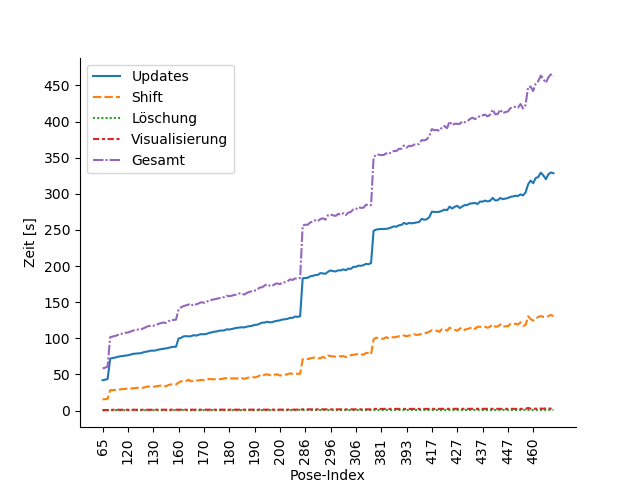
\includegraphics[width=1.0\linewidth]{GlobalMapUpdateTime}
  		 \centering \caption{}
  		 \label{fig:GlobalMapUpdateTime}
	\end{subfigure}%
	\begin{subfigure}{.5\textwidth}
    	\centering
  		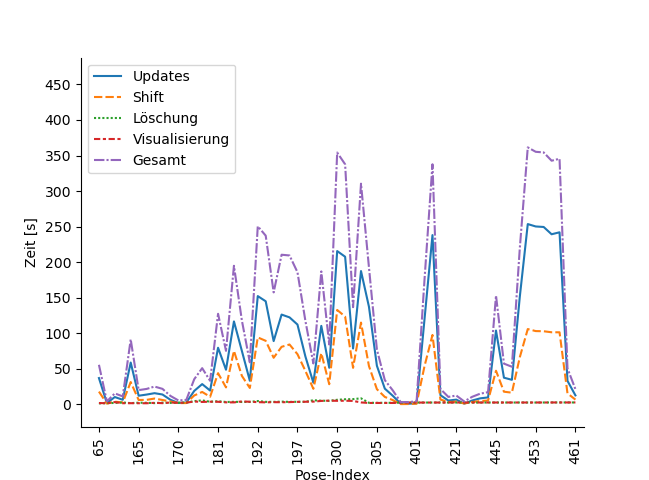
\includegraphics[width=1.0\linewidth]{PartialMapUpdateTime}
  		\centering \caption{}
  		\label{fig:PartialMapUpdateTime}
	\end{subfigure}
	\caption{Grafischer Vergleich der Laufzeiten des globalen und partiellen Updates auf Basis des vorgestellten Hannover-1 Datensatzes. Dargestellt sind die Laufzeiten für jedes einzelne durchgeführte Update. Zusätzlich wurden kenntlich gemacht, wie sich welche Komponenten der Updates auf die Laufzeit auswirken. Die Laufzeit des globalen Updates ist links, die des partiellen rechts abgebildet. Es ist deutlich zu erkennen, dass die Laufzeit im globalen Update stetig ansteigt. Sprünge in diesem Graphen entstehen durch Teilbereiche des Pfades, in denen keine Schleifen geschlossen wurden und entsprechend kein Update der Karte nötig ist. Im Graphen, der die Laufzeit des partiellen Updates beschreibt sind starke Sprünge zu beobachten. Dies liegt an der variablen Anzahl nötiger Löschungen und TSDF-Updates, basierend auf den angegebenen Schwellen, anhand derer bestimmt wird, ob ein Update durchgeführt wird. Hier betragen diese Schwellen in der Translation $3,2 cm$ und in der Rotation $2^\circ$. In der Gesamtheit benötigt das globale Karten-Update für den Hannover-1 Datensatz mit $468$ Posen $13.2h$, während das partielle Update $1.96h$ benötigt. Dies entspricht einer Verringerung der Laufzeit auf $15\%$ der Laufzeit der vorgegebenen Base-Line in Form des globalen Updates. Diese Verringerung gründet sich in der Verringerung der Laufzeiten der einzelnen Bestandteile des Algorithmus durch eine geringere Anzahl an Posen, die an einem Update beteiligt sind. In einigen Fällen reduziert sich diese Anzahl sogar auf $0$. Dementsprechend ist vorstellbar, dass in einem optimalen Datensatz mit regelmäßigen Schleifenschlüssen, die nur eine geringe Auswirkung auf den Verlauf des Pfades haben nur sehr wenige oder nahezu keine Updates durchzuführen sind, während beim naiven globalen Update nach jedem Schleifenschluss ein Update durchgeführt wird, ohne Berücksichtigung der genannten Fälle. Die durchschnittliche Zeit, die das Update pro Pose gemäß dieser Daten benötigt, beträgt $0.91s$.}
	\label{fig:MapUpdateTimes}
\end{figure}
	
Im Folgenden werden die Ergebnisse des partiellen Updates mit denen des globalen Updates durch einen Vergleich der TSDF evaluiert. Dazu wird ein in \cite{HATSDF} implementierter Ansatz zur Rekonstruktion der Oberfläche aus TSDF-Karten in Form eines Dreiecksnetzes verwendet. Dies ergibt sowohl für das globale, als auch für das partielle Update ein Dreiecksnetz bestehend aus \emph{Vertices (Knoten)} und \emph{Faces (Flächen, hier Dreiecksflächen)}. Mit Hilfe der Software CloudCompare \cite{cloudcompare} können die Punktwolken der beiden resultierenden Meshes miteinander verglichen werden. Dieser Vergleich ist in Abbildung \ref{fig:CloudDifferences} als Vergleich der berechneten absoluten Distanzen zwischen den Punktwolken dargestellt.


\begin{figure}
	\centering
	\begin{subfigure}{.5\textwidth}
		 \centering
  		 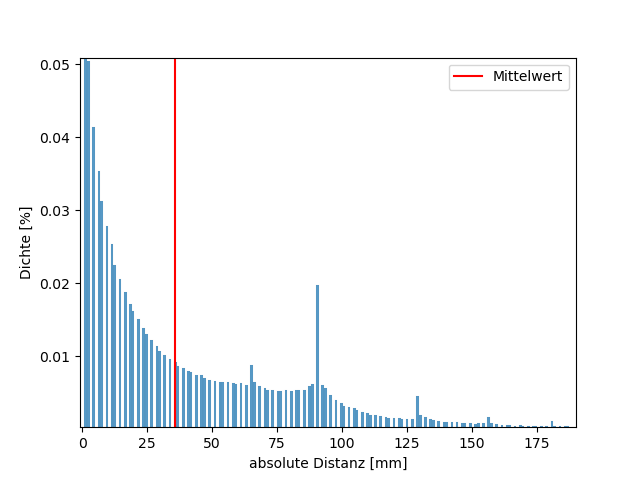
\includegraphics[width=1.0\linewidth]{HistogramCCphysik128_seaborn_fixed}
  		 \centering \caption{Absolute Distanzen näherster Punkte zwischen den aus dem Dreiecksnetzen des partiellen und globalen Update extrahierten Punktwolken.}
  		 \label{fig:HistogramCCphysik128_seaborn}
	\end{subfigure}%
	\begin{subfigure}{.5\textwidth}
    	\centering
  		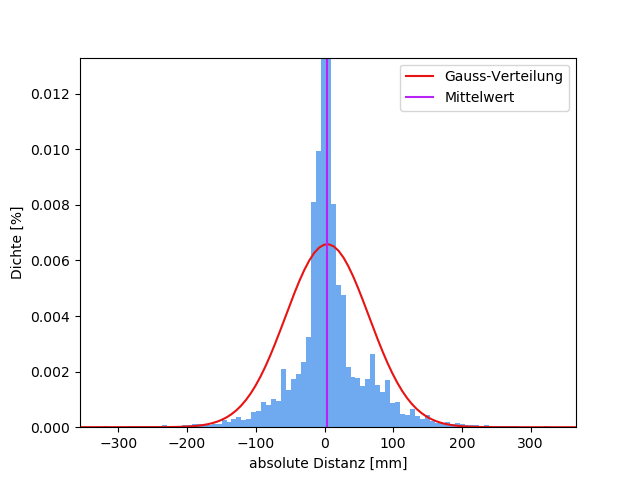
\includegraphics[width=1.0\linewidth]{Histogram_point_to_mesh}
  		\centering \caption{Absolute Distanz zwischen den Punktdaten der Punktwolke des partiellen Updates, extrahiert aus dem zugehörigen Dreiecksnetz und dem Dreiecksnetz des globalen Updates.}
  		\label{fig:Histogram_point_to_mesh}
	\end{subfigure}
	\caption{Die hier dargestellten Histogramme zeigen die Verteilungen der absoluten Distanzen zwischen den vorgestellten Methoden zum Update der TSDF-Karte. Verglichen ist jeweils der partielle Ansatz im Vergleich mit dem globalen Ansatz. Die absoluten Distanzen ergeben sich aus der Identifikation der Distanzen der aus den generierten Dreiecksnetzen extrahierten Punktwolken zu den nächsten Punkten der zu vergleichenden Punktwolke. Bei den Verteilungen handelt es sich nicht um Normalverteilungen, sie ähneln viel mehr einem exponentiellen Abfall. Aus diesem Grund werden an dieser Stelle nicht die Parameter von Normalverteilungen, sondern lediglich der Mittelwert der Verteilungen berechnet, der als rote vertikale Linie in den Abbildungen dargestellt ist. Im linken Teil der Abbildung ist die Verteilung für den in Kapitel \ref{chapter:loop_closure} vorgestellten Datensatz der Universität Osnabrück dargestellt, im rechten Teil der Abbildung die Verteilung für den Hannover-1 Datensatz. Der Mittelwert der linken Verteilung beträgt $35.89mm$ und der der rechten $mm$. Dies macht deutlich, dass zwar ein Unterschied zwischen den Ergebnissen der betrachteten Update-Verfahren besteht, dieser aber im Schnitt deutlich geringer ist, als die in beiden Datensätzen verwendete TSDF-Zellgröße mit einer Seitenlänge von $128mm$. Dabei stellt die Zellgröße den begrenzenden Faktor für die Genauigkeit der Ergebnisse dar.}
	\label{fig:CloudDifferences}
\end{figure}



Nachfolgendes Kapitel fasst die Ergebnisse der Arbeit zusammen und liefert einen Ausblick über mögliche zukünftige Arbeiten im Themengebiet dieses Projektes.


